\documentclass{standalone}
\usepackage{tikz}
\usetikzlibrary{arrows.meta, positioning}

\begin{document}

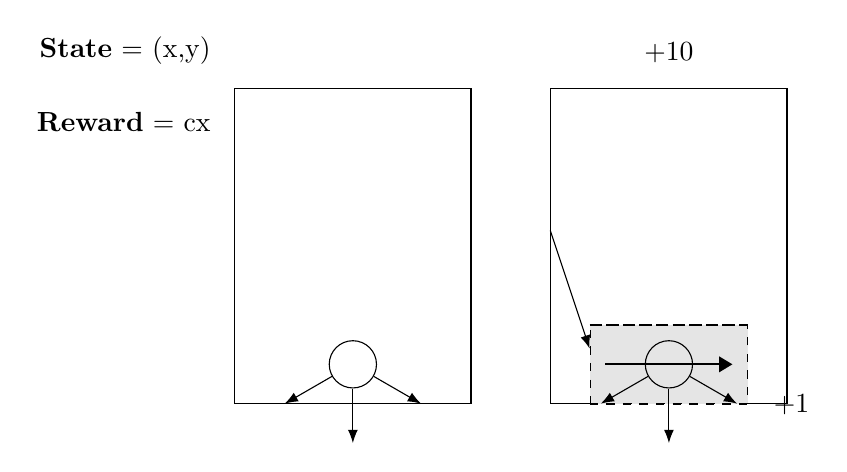
\begin{tikzpicture}[node distance=1cm, >=Latex]

% Left panel
\node[draw, minimum width=3cm, minimum height=4cm] (leftbox) {};
\node[above left=0.5em and 0.5em of leftbox.north west] {\textbf{State} = (x,y)};
\node[below left=0.5em and 0.5em of leftbox.north west] {\textbf{Reward} = cx};

% State circle and arrows
\node[circle, draw, inner sep=2pt, minimum size=6mm] (state1) at ([yshift=-1.5cm]leftbox.center) {};
\draw[->] (state1) -- ++(0,-1cm);
\draw[->] (state1) -- ++(-0.866cm,-0.5cm); % Left arrow
\draw[->] (state1) -- ++(0.866cm,-0.5cm);  % Right arrow

% Right panel
\node[draw, minimum width=3cm, minimum height=4cm, right=1cm of leftbox] (rightbox) {};

% Top label
\node[above=0.2cm of rightbox.north] {$+10$};

% Treadmill rectangle and state
\node[draw, minimum width=2cm, minimum height=1cm, dashed, fill=gray!20] (treadmill) at ([yshift=-1.5cm]rightbox.center) {};
\node[circle, draw, inner sep=2pt, minimum size=6mm] (state2) at (treadmill.center) {};
\node[right=0.2cm of treadmill.south east] {$+1$};

% Treadmill movement arrows
\draw[dashed, thick] ([yshift=0.5cm]treadmill.west) -- ([yshift=0.5cm]treadmill.east);
\draw[dashed, thick] ([yshift=-0.5cm]treadmill.west) -- ([yshift=-0.5cm]treadmill.east);
\draw[-Triangle, thick] ([xshift=0.2cm]treadmill.west) -- ([xshift=-0.2cm]treadmill.east);

% Arrows extending from the state
\draw[->] (state2) -- ++(0,-1cm);
\draw[->] (state2) -- ++(-0.866cm,-0.5cm); % Left arrow
\draw[->] (state2) -- ++(0.866cm,-0.5cm);  % Right arrow

% Connection line to treadmill
\draw[->] ([yshift=0.2cm]rightbox.west) -- ([yshift=0.2cm]treadmill.west);

\end{tikzpicture}

\end{document}